\documentclass[
	parskip=half,10pt,
	numbers= noenddot, % enddot -> Ebenen mit Punkt abschließen -> 1.1., noenddot -> ohne Punkt
	toc=flat, % TOC in Tabellenform (bei langen Überschrtiften verwenden)
	oneside,
	twocolumn,
	]{scrartcl}



\usepackage[T1]{fontenc} % verwende Type 1 - Zeichensatz
\usepackage{libertine}
\usepackage[scaled=0.78]{beramono} %Schreibmaschinenschrift
\usepackage{microtype}
\usepackage[utf8]{inputenc}
\usepackage[english]{babel} % internationale Sprachunterstützung



\usepackage{amsmath}
\usepackage{amssymb}
\usepackage{amsthm}
\usepackage{tabularx}
\usepackage{booktabs}
\usepackage{longtable}
\usepackage{rotating} % Rotationen, Reflexionen, ...
\usepackage{multido} % Wiederholungen
\usepackage{wrapfig}
\usepackage{todonotes}
\usepackage{siunitx} %\si units
\usepackage{units}
\usepackage{icomma} %keine Leerzeichen nach Komma im mathmode
\usepackage[numbers,sort]{natbib}
\usepackage{babelbib} %deutsche bibliographie
\usepackage{multirow}
\usepackage{rotating}
\usepackage{url}

\usepackage{tikz}
\usepackage{float}
\usepackage{pgfplots}
%\pgfplotsset{compat=1.8}
\usepackage{caption}
\usepackage{graphicx}
\usepackage{subcaption} %für subfigures
\captionsetup{labelfont={bf,sf},format = plain, textfont=sf}
%\usepackage{asymptote}
\usepackage{ragged2e}
\usepackage[bottom]{footmisc}
\usepackage{csquotes} %Anführungszeichen
\usepackage[ngerman]{varioref} % Zum komfortablen Verlinken



\usepackage{geometry}
\geometry{a4paper,lmargin=2.5cm, rmargin=2.5cm, tmargin=2.5cm, bmargin=3cm, marginparwidth=3cm, marginparsep=1em}


\usepackage{fancyhdr}
\pagestyle{fancy}
\renewcommand\footrulewidth{0.5pt}
\fancyhf{}
\lhead{\leftmark}

\fancyfoot{}
\rfoot{\thepage}
\lfoot{Till Kolster \& Lukas Schmidt}


\usepackage{layout}

\usepackage[%draft
linkbordercolor=blue,
colorlinks,
linkcolor=blue,
linktocpage,
linktoc=all]{hyperref} % IMMER AM ENDE

%\setkomafont{subparagraph}{\mdseries\itshape}
\setcounter{secnumdepth}{3}%Bis zu welcher Ebene nummeriert werden soll. 
\setcounter{tocdepth}{2}%Bis zu welcher Tiefe ins TOC soll.

%%%%%EIGENE DEFINITIONEN%%%%%

\newcolumntype{Y}{>{\RaggedRight\hspace{0pt}} X }
\newcommand\Grad{$^\circ$}
\newcommand\HAND{\marginnote{\Large\vreflectbox{\ding{43}}}\xspace}%\newcommand\Name{Befehlsdifinition}
\newcommand\MPAR[1]{
\marginnote[\RaggedLeft#1]{\RaggedRight#1}}
% \hspace{0pt} entspricht dem ersten (nicht sichtbaren) Wort
\newcolumntype{P}[1]{>{\RaggedRight\hspace{0pt}}p{#1}}
\newcolumntype{R}{>{\tiny}r}

\pgfmathdeclarefunction{gauss}{4}{%
  \pgfmathparse{#1*exp(-((x-#2)^2)/(2*#3^2))+#4}%
}


\title {Rayleigh-Scattering}
\author {Till Kolster \thanks{Freie Universität Berlin} \and Lukas Schmidt \thanks{Freie Universität Berlin}}


\begin{document}

\begin{titlepage}

\vspace*{-2cm}

\vspace{6cm}
\begin{center}
\huge \bfseries
Fortgeschrittenen-Praktikum -- Rayleigh-Scattering

\vspace{0.5cm}
\large \bfseries
03.12.2014

\vspace{1.5cm}

\large\normalfont von

\bigskip
\textbf{Till Kolster \& Lukas Schmidt}

\bigskip
Tutor: Dr. Andrey Pivtsov

\vspace{3cm}

\parbox{0.8\linewidth}{%
\textit{This experiment was done within the scope of the advanced lab course for Bachelor Students at Freie Universität Berlin.
It should give an experimental introduction to Rayleigh scattering processes, the Scattering-Ring-Down Spectroscopy and should
give a better understanding of Rayleigh scattering phenomenon in nature.
}}


\end{center}
\end{titlepage}

\section{Introduction}

The scattering process is a precess where electromagnetic waves interact with particles and change their direction. By understanding this process one can 
explain the color of the sky and other interesting phenomena. The Rayleigh-scattering observed in this experiment was first postulated by John William Strutt, 3rd 
Baron of Rayleigh and was confirmed experimentally later. The greater Theory to describe such phenomena is the Lorenz-Mie-scattering theory, which 
describes elastic scattering at non-conductive spheres of different sizes. In the case of air-molecules, the scattering strongly depends on the wavelength. 


\section{Theoretical Principles}

Rayleigh Scattering is a type of elastic scattering of electromagnetic waves at particles, which are significantly smaller than the wavelength of the photon. 
Rayleigh-scattering can be explained by the Mie-theory, which explains the dependence of the scattering-process from the wavelength. 

If there is a collision of an electromagnetic wave with an atom, the atom will be subject of a change of the electromagnetic field produced by the photon. 
This change will be sinusoidal and hence the atom will resonate. Therefore, the atom can be described as a dipole. 
The electric and magnetic dipole field can be described the following way\cite{griffiths}:
\begin{align}
\vec{E}(\vec{r},t) &= -\frac{\mu_0 p_0 \omega^2}{4 \pi}  \frac{\sin\theta}{r} \cos \left ( \omega \left (t-\frac{r}{c}\right ) \right )\hat{e}_{\theta} \\
\vec{B}(\vec{r},t) &= -\frac{\mu_0 p_0 \omega^2}{4 \pi}  \frac{\sin\theta}{r} \cos \left ( \omega \left (t-\frac{r}{c}\right ) \right )\hat{e}_{\phi},
\end{align}
where $\omega$ is the dipole-frequency and $p_0$ the dipole-moment. 
The probability that a scattering process will take can be described by the scattering cross-section $\sigma$:
\begin{align}
\sigma(\nu) &= \frac{8 }{3} \pi \frac{e^2}{m_e c^2} \frac{\nu^4}{\omega^4},
\end{align}
where $\nu$ is the frequency of the wave. Since (in our case) we have oscillating atoms, $\omega \ll \nu$, because $\lambda \gg$ size of the atom. 
We may replace $\nu= \nicefrac{c}{\lambda}$ to get the dependence of the wavelength. 
In the case of several atoms $N$ and the resulting refraction-index $n$ we can rewrite $\sigma$ as:
\begin{align}
\sigma (\lambda) &= \frac{8 \pi (n^2 -1)^2}{3 N^2 \lambda^4}
\end{align}
With this scattering-cross-section it is easy to get the scattering factor  $\beta$:
\begin{align}
\beta &= N \sigma = \frac{8 \pi (n^2 -1)^2}{3 N \lambda^4}
\label{eq:betatheo}
\end{align}
With the dependence of $\lambda^4$ the colors of the sky can be explained: Taking a sunset or sunrise it can be observed that the sky appears red in the direction of the sun and blue in other directions. This is because sunlight gets scattered while passing the atmosphere and especially the troposphere. As photons with larger $\lambda$ have a lower cross-section and therefore a lower probability to get scattered, more of these photons arrive on the direct way from the sun to the earth as the more energetic ones. These more energetic photons with smaller $\lambda$ have a higher probability to get scattered and arrive at the observer on the earth especially in the indirect way and turn the sky blue.
\section{Cavity Ring-Down Spectroscopy}

To measure the Rayleigh-scattering, in this experiment a cavity-ring-down-spectrometer ist used. 
\begin{figure}[h]
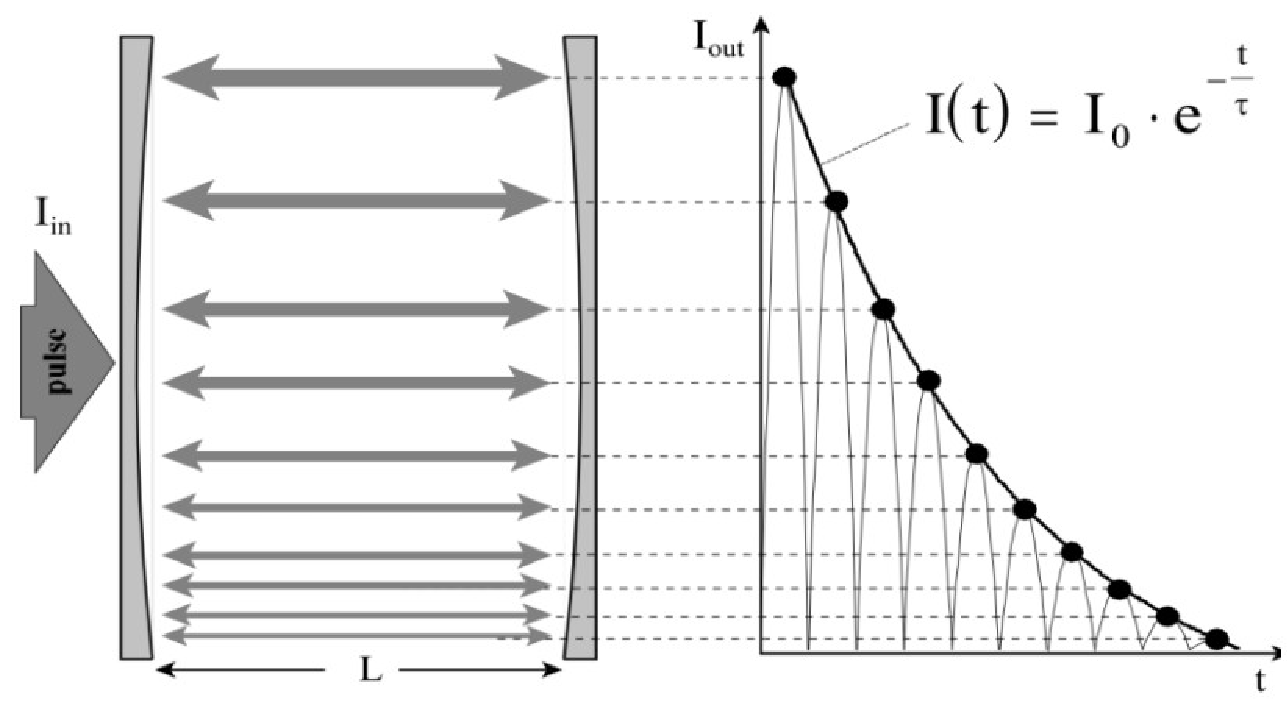
\includegraphics[width=.48 \textwidth]{images/crds.pdf}
\caption{Schematic set-up of a cavity-ring-down-spectrometer \cite{wiki}}
\label{fig:set-up}
\end{figure}
The cavity-ring-down-spectrometer is made of two spherical mirrors and a tube, which can be evacuated. A laser-beam is introduced into the cavity and may be reflected 
several times, to maximize the length of interaction with the medium in the cavity. This way, scattering with a very small number of particles can be measured. 
The reflectance of the mirrors is at about $R=99.98 \%$, so each time the beam hits one of the mirrors about $0.02\%$ of the light is 
transmitted. Behind one of the mirrors is a detector which measures the transmitted part of the beam. The signal intensity $I$ which is recorded this way is 
decreasing exponentially with the time $t$. This is caused by two different mechanisms: Scattering and reflection:
\begin{align}
I(t) &= I_0 e^{-\frac{t}{\tau}}=I_0 e^{- t \left ( \beta c + \frac{1}{\tau_0} \right )},
\label{eq:IDec}
\end{align}
where $I_0$ is the starting intensity and $\tau_0$ the damping by reflection. It can be expressed the following way:
\begin{align}
\tau_0 &= \frac{L}{c(1-R)},
\end{align}
with $L$ the length of the cavity. This is the damping, when the cavity is evacuated. If a gas is introduced, we get:
\begin{align}
\tau(t) &= \frac{L}{c(1-R(\lambda) + \beta(\lambda)L)}
\end{align}
By comparison of the damping constant in the evacuated and the non-evacuated case, the coefficient $\beta$ can be calculated. 
\section{Set-up}
To measure the Rayleigh scattering we had a set-up as follows:
\begin{figure}[h]
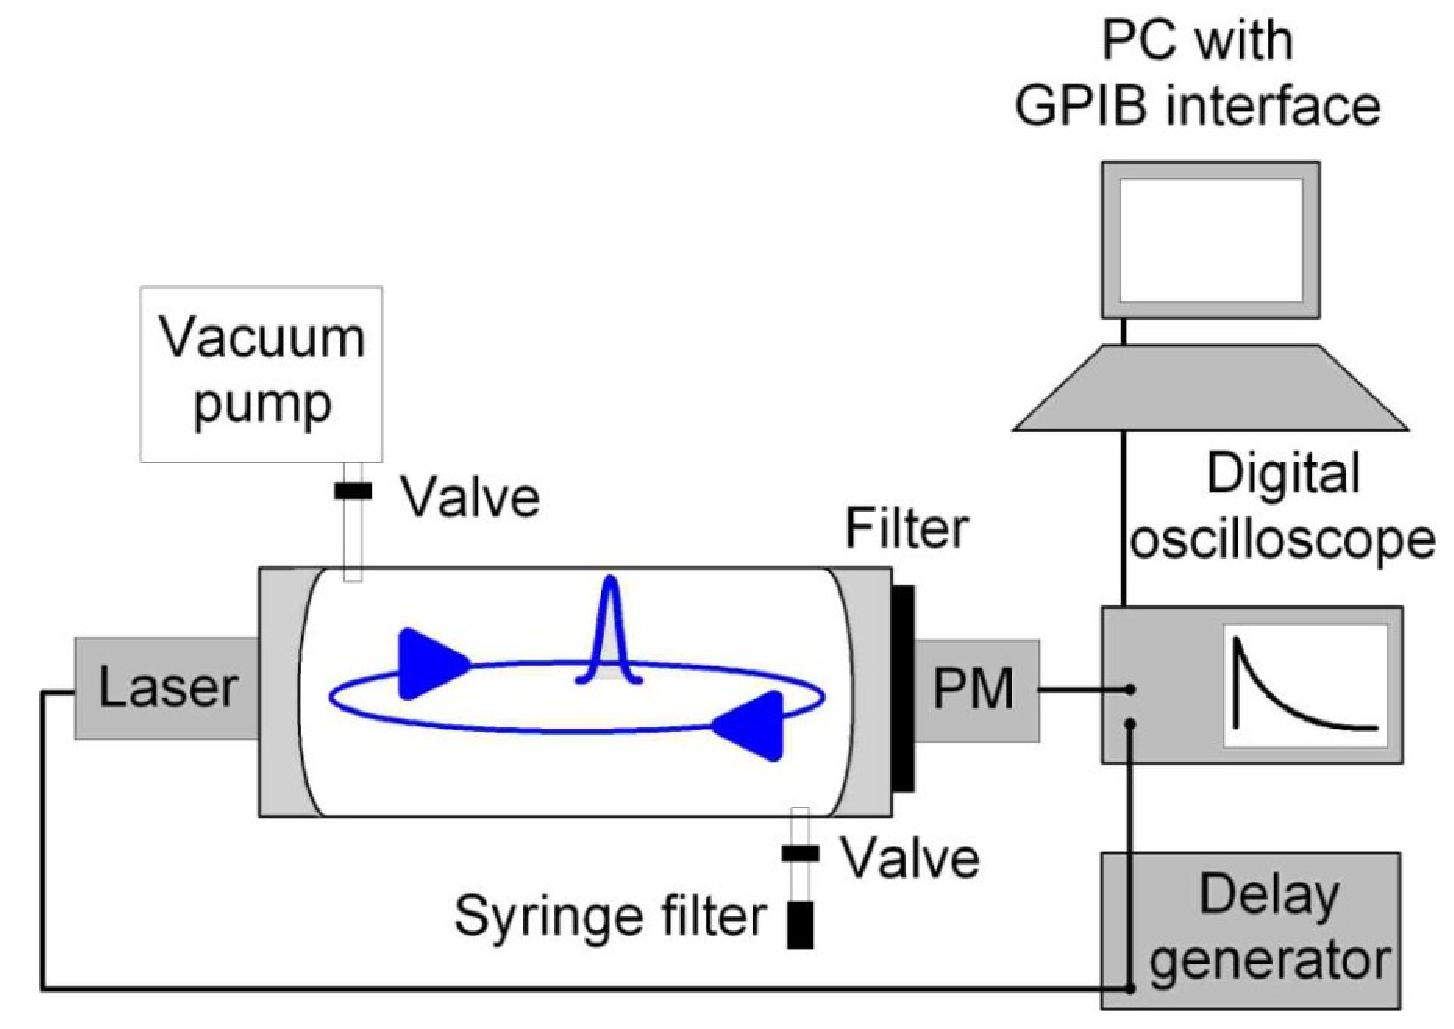
\includegraphics[width = .48 \textwidth]{images/aufbau.pdf}
\caption{Set-up of the experiment \citep{wiki}}
\label{fig:experiment}
\end{figure}

\section{Description of measurement}
The experiment was started with an already evacuated cavity. The quality of the vacuum was observed by an analogue manometer. It was assumed, that a vacuum of sufficient 
quality was reached, when the indicator of the manometer hit the lowest position possible. 
To adjust the system we used the green laser. The green laser was chosen as the mirrors in the cavity are less reflective for green light and the green light is easier to 
see with bare eyes. The set-up was adjusted by changing the position and the vertical angle of the laser until the laser hit every iris diaphragm centrally. In a next step 
the laserbeam that exits the cavity was centralised and afterwards the reflection of the laser was set to overlap with the source by changing the position of the mirrors. 
After the alignment has led to the desired light path, the green laser was replaced by the violet one with $\lambda=405\si{\nano \meter}$ with whom the measurements were 
made, as the Rayleigh effect is higher with small $\lambda$ and the mirrors are optimized for this wavelength. After a short warm up period, the power of the laser could be 
regulated at the computer and was set to 2mW for the adjustments. As the position of the beam of the violet laser is not at the same position as the green one, the 
adjustments of its position had to be repeated while letting the position of the mirrors untouched.

The photomultiplier was switched on and turned to the highest sensitivity. With the adjustment-screws of the mirrors their direction was changed until the decaying time 
which could be observed via the oscilloscope was maximal.

The power of the laser was increased up to $75\si{\milli \watt}$ to be able to decrease the sensitivity of the photomultiplier and to obtain a better signal with less noise.
On the computer we measured the signal multiple times trying to prolong the decaying times each time. As software we used LabView that was able to show the decaying time 
very easily. The values for the decaying times didn't reach the estimated values of about $11\cdot 10^{-6}\si{\second}$. The maximum value in the case with vacuum was 
at about $9.5\cdot 10^{-6}\si{\second}$.
As no greater values for the decay time were reached after several readjustments, the valve of the cavity was opened and atmosphere pressure established with filtered air. 
By the changing pressure the position of the mirrors has changed, so it was needed to readjust them with the adjustment-screws.
New decaying times were measured that were shorter than the measured values we had before which was expected as Rayleigh scattering in the air occurs in this set-up.
In the end vacuum was re-established to use the resting time to reach longer ring-down-times. But the measured values didn't exceed the previous values measured in 
vacuum. Values for temperature and time of each data acquirement can be found in the transcription of the protocol in the annex.


\section{Evaluation}
For the evaluation the measured data was imported in Mathematica 10 and analysed by fitting the decaying curve. A notebook is attached to make the results reproducible.
Measurements in vacuum led to the curve in Fig. \ref{fig:vacuum}. We chose the measurement row with the highest decaying time which should correspond to the best alignment 
of mirrors, cavity and laser. 

\begin{figure}[h]
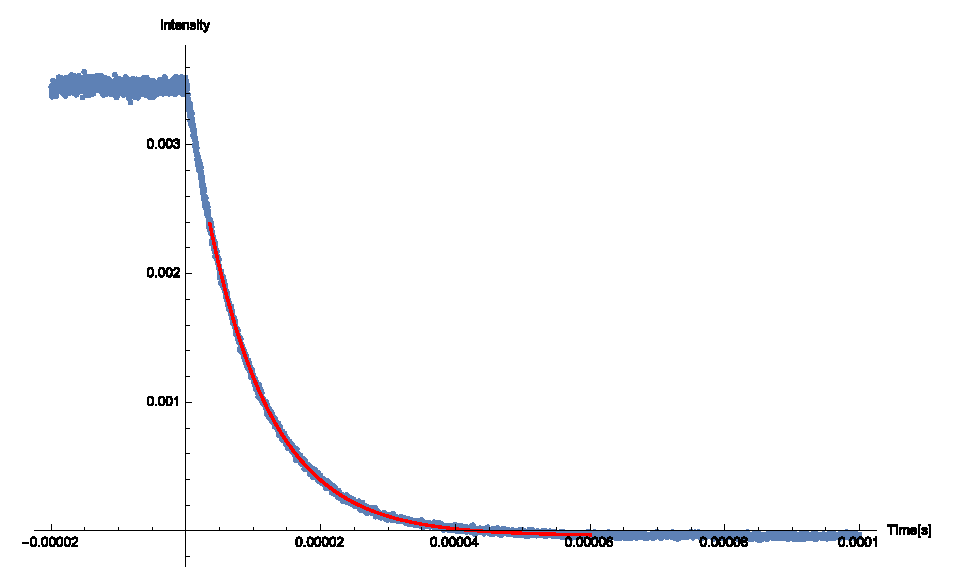
\includegraphics[width=\textwidth/2]{images/vacuum.eps}
\caption{Decaying signal with evacuated cavity - measurement row at 2:43pm}
\label{fig:vacuum}
\end{figure}

Mesurements with air led to the curve that can be seen in Fig. \ref{fig:air}

\begin{figure}[hb]
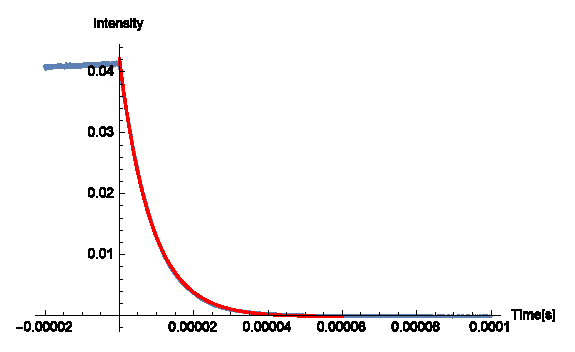
\includegraphics[width=\textwidth/2]{images/air.eps}
\caption{Decaying signal with cavity filled with air at atmosphere pressure - measurement row at 2:50pm}
\label{fig:air}
\end{figure}
\begin{figure}
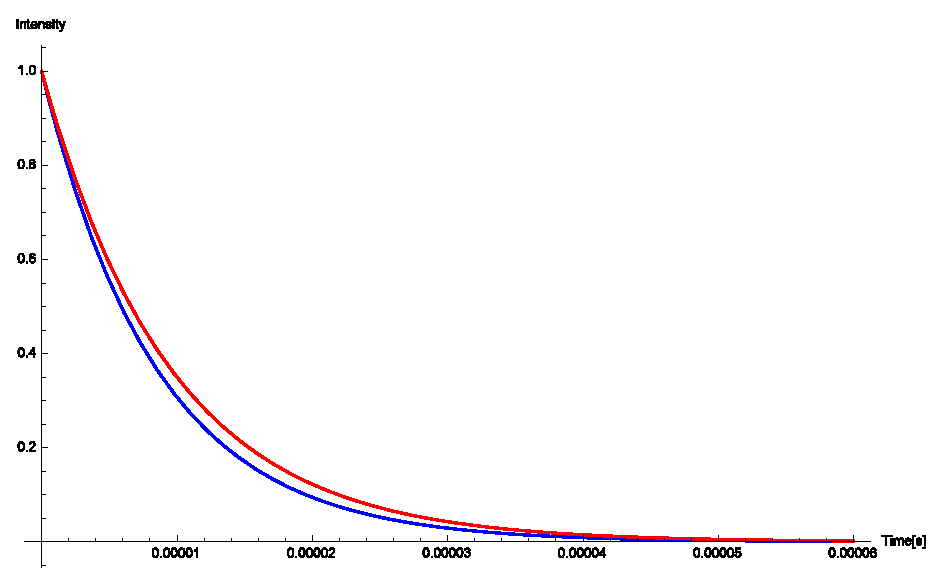
\includegraphics[width=\textwidth/2]{images/airvacuum.eps}
\caption{Both fits: Vacuum in red and the case with air in blue }
\label{fig:airvacuum}
\end{figure}

From the fit, values for the decaying times were determined. Both fits together can be seen in figure \ref{fig:airvacuum}.
The decaying time in vacuum was found at $\tau_0=(9.517\pm0.006)\cdot 10^{-6}s$. The decaying time with 
air is $\tau=(8.470\pm0.005)\cdot 10^{-6}s$. The error values correspond to the error of finding the fit. 
With the determined values for $\tau$ and $\tau_0$ a value for $\beta$ can be derived from formula \ref{eq:IDec}.

\begin{align}
\beta=\frac{1}{c}\left(\frac{1}{\tau}-\frac{1}{\tau_0}\right)=(4.328\pm0.032)\cdot 10^{-5}\si{\meter}^{-1}
\end{align}
Calculation of the theoretical value of $\beta$ with formula \ref{eq:betatheo} needs values for $n$ and $N$. Refraction index $n$ was calculated using the modified 
Edlén equation which leads, using the measured values for p and T and an estimated relative humidity of $50\%$, to a value of $n=1.00028152$\cite{edlen}
The number of particles per cubic meter was determined using the ideal gas equation:
\begin{align}
N=\frac{p}{k_B\cdot T}
\end{align}

\begin{align}
\beta &= \frac{8\cdot \pi^3\cdot (n^2-1)^2}{3 N \lambda^4} \\ & =(3.834\pm0.013)\cdot 10^{-5}\si{\meter}^{-1}
\end{align}

\section{Summary and Discussion}
Decaying times were determined through fitting the intensity decay after each laser pulse. 
In vaccuum:
\begin{align}
\tau_0=(9.52\pm0.01)\cdot 10^{-6}s
\end{align}
and with air:
\begin{align}
\tau=(8.47\pm0.01)\cdot 10^{-6}s
\end{align}
With these values an experimental value of the scattering factor could be determined: 
\begin{align}
\beta=(4.33\pm0.04)\cdot 10^{-5}\si{\meter}^{-1}
\end{align}
The theoretical value for the scattering factor is
\begin{align}
\beta=(3.83\pm0.02)\cdot 10^{-5}\si{\meter}^{-1}
\end{align}
The order of magnitude is the same, but taking only the uncertainty of the fit into account the values are significantly different.
The highest error comes from the alignment of the experimental set-up. Already small changes result in different decaying values. In our case the deviation of the 
experimental value is very likely caused by a better optimized alignment for vacuum as for the set-up with air. As the alignment changes when atmosphere pressure is 
re-established in the cavity, the alignment has to be readjusted and therefore is not the same.
The sensibility to the adjustment can be observed when fitting other measuring rows. Even negative $\beta$ can be obtained or scattering factors of 
$\beta\approx 6 \cdot 10^-5\si{\meter}^{-1}$
This stresses the importance of optimizing both cases equally.

The conclusion that could be drawn is, that the experiment is suitable to get an idea of the order of magnitude of the scattering factor. For measuring exact values, a 
way has to be found to ensure that measurements take place under same conditions.

\section{Protocol}
Times correspond to the computer time which had a difference of 15min to realtime.

Temperature: $T=(18.5\pm 0.5)^\circ C$

Atmosphere pressure: $p=1023.4\si{\hecto \pascal}$\cite{wetter}

The values were measured/looked up at the beginning of the experiment.

In the following list, each time refers to a measuring row. Normally the experimental set-up was optimized between each data acquirement. Only if the oscilloscope hasn't collected enough data for the average yet and the set up seems to be worth to save the data, the same measurement was repeated.
No description of the time means that the main parameters weren't changed from the measurements before and only the set-up was optimized. 
\subsection*{Evacuated cavity}  
\begin{description}
\item[13:45] Laser: $5\si{\milli \watt}$
\item[13:53]
\item[13:54]
\item[13:55] Changed power of laser to $20\si{\milli \watt}$
\item[14:00] Using Average, Laser still $20\si{\milli \watt}$
\item[14:07] Average over 1024
\item[14:10]
\item[14:16] Changed power of laser to $50\si{\milli \watt}$
\item[14:18]
\item[14:21] Average not reached
\item[14:22] Average over 1024 reached
\item[14:25]
\item[14:30] Changed power of laser to $75\si{\milli \watt}$, Average not reached
\item[14:32] Average reached
\item[14:36] Average not reached
\item[14:42] Average not reached
\item[14:43] Average reached
\end{description}
\subsection*{Cavity filled with air}
\begin{description}
\item[14:49] Laser: $75\si{\milli \watt}$, Average 1024 not reached
\item[14:50] Average reached
\item[14:53]
\end{description}
\subsection*{Evacuated cavity}
\begin{description}
\item[15:07]
\item[15:15]
\item[15:19]
\item[15:20]
\item[15:26]
\item[15:27]
\item[15:32]
\item[15:33]
\item[15:35]
\end{description}
\newpage
\bibliographystyle{unsrtnat}
\bibliography{raybib}

\end{document}





